%%%%%%%%%%%%%%%%%%%%%%%%%%%%%%%%%%%%%%%%%%%%%%%%%%%%%%%%%%%%%%%%%%%%%%%%
%
%   SMT-COMP 2021 - Presentation on SMT-Workshop
%                   virtual conference in "Los Angeles"
%
%   1 hour
%
%%%%%%%%%%%%%%%%%%%%%%%%%%%%%%%%%%%%%%%%%%%%%%%%%%%%%%%%%%%%%%%%%%%%%%%%

\documentclass[table]{beamer}
\usepackage[utf8]{inputenc}
\usepackage{xcolor}
\usepackage{tikz}
\usetikzlibrary{shapes,shapes.callouts,automata,trees}
\usetikzlibrary{decorations.pathmorphing,external,fit}
\usetikzlibrary{calc}
\usetikzlibrary{backgrounds} %used for the CEGAR figure
\usepackage{amssymb}
\usepackage{clrscode}
\usepackage{pifont}
\usepackage{pdfpages}
\geometry{papersize={16cm,9cm}}
%\tikzexternalize

\colorlet{MYred}{red!70!black}
\definecolor{MYgreen}{rgb}{.1,.5,0}
\definecolor{MYblue}{rgb}{0,.42,.714}
\colorlet{MYgray}{white!95!MYblue}
\colorlet{MYorange}{orange!80!black}
\definecolor{gold}{rgb}{.8,.6,0}
\colorlet{silver}{white!55!black}
\colorlet{bronze}{brown!70!black}
\def\tick{\ding{52}}
\def\cross{\ding{54}}

%%%%%%%%%%%%%%%%%%%%
%%% Beamer stuff %%%
%%%%%%%%%%%%%%%%%%%%
\usetheme{default}
\useinnertheme{rounded}
\setbeamertemplate{frametitle}[default][center]
\setbeamertemplate{footline}{\quad\hfill\footnotesize\insertframenumber\strut\kern1em\vskip2pt}
\setbeamertemplate{navigation symbols}{}
\setbeamertemplate{itemize/enumerate subbody begin}{\normalsize}
\usefonttheme[onlymath]{serif} % Nicer formulas
\setbeamercolor{block body}{bg=black!10}
\setbeamercolor{block title}{bg=black!20}

\AtBeginSection[]{
  \begin{frame}
  \vfill
  \centering
  \begin{beamercolorbox}[sep=8pt,center,shadow=true,rounded=true]{title}
    \usebeamerfont{title}\insertsectionhead\par%
  \end{beamercolorbox}
  \vfill
  \end{frame}
}

\def\emph#1{\textcolor{MYblue}{#1}}

%%% Titel, Autor und Datum des Vortrags:
\title{SMT-COMP 2022\\
17th International Satisfiability Modulo Theory Competition}
\author{\emph{Haniel Barbosa} \and Jochen Hoenicke \and Fran\c{c}ois Bobot}
\date{Aug 9, 2022\\[2ex]      \includegraphics[width=\textwidth]{floc}
}

%% Institut
\institute{
  Universidade Federal de Minas Gerais, Brazil \and
  Albert-Ludwigs-Universit\"at Freiburg, Germany \and
  CEA List, France
}


%%%%%%%%%%%%%%%%%%%%%%%%%%%%%%%
% MACROS

% database symbol (from stackexchange)

\makeatletter
\tikzset{
    database/.style={
        path picture={
            \draw (0, 1.5*\database@segmentheight) circle [x radius=\database@radius,y radius=\database@aspectratio*\database@radius];
            \draw (-\database@radius, 0.5*\database@segmentheight) arc [start angle=180,end angle=360,x radius=\database@radius, y radius=\database@aspectratio*\database@radius];
            \draw (-\database@radius,-0.5*\database@segmentheight) arc [start angle=180,end angle=360,x radius=\database@radius, y radius=\database@aspectratio*\database@radius];
            \draw (-\database@radius,1.5*\database@segmentheight) -- ++(0,-3*\database@segmentheight) arc [start angle=180,end angle=360,x radius=\database@radius, y radius=\database@aspectratio*\database@radius] -- ++(0,3*\database@segmentheight);
        },
        minimum width=2*\database@radius + \pgflinewidth,
        minimum height=3*\database@segmentheight + 2*\database@aspectratio*\database@radius + \pgflinewidth,
    },
    database segment height/.store in=\database@segmentheight,
    database radius/.store in=\database@radius,
    database aspect ratio/.store in=\database@aspectratio,
    database segment height=0.1cm,
    database radius=0.25cm,
    database aspect ratio=0.35,
}
\makeatother


%%%%%%%%%%%%%%%%%%%%%%%%%%%%%%%

\newcommand{\yell}[1]{{\color{red} [#1]}}

% 2952bfff
\definecolor{ceruleanblue}{rgb}{0.16, 0.32, 0.75}

\newcommand\vitem{\vfill\item}

\begin{document}

\begin{frame}
  \titlepage
\end{frame}


\begin{frame}
  \frametitle{SMT-COMP}

  \begin{minipage}[b]{.6\textwidth}
    Annual competition for \emph{SMT solvers}\\
    on (a selection of) benchmarks from \emph{SMT-LIB}
  \end{minipage}%
  \begin{minipage}{.4\textwidth}
    \begin{block}{History}
      \begin{tabular}{rp{3cm}}
        \textbf{2005} & first competition \\
        \textbf{2013} & evaluation instead \\
        & of competition\\
        \textbf{2014} & since then hosted\\
        & by \emph{StarExec}
      \end{tabular}
    \end{block}
  \end{minipage}

  Goals:
  \begin{itemize}
  \item spur development of SMT solver implementations
  \item promote SMT solvers and their usage
  \item support the SMT-LIB project
    \begin{itemize}
    \item to promote and develop the SMT-LIB format
    \begin{itemize}
      \item model validation
      \item proof checking
    \end{itemize}
    \item to collect relevant benchmarks
    \end{itemize}
  \item engage and include new members
  \end{itemize}

\end{frame}



\begin{frame}
  \frametitle{SMT Solvers and SMT-LIB}
  SMT Solver
  \begin{itemize}
  \item checks formulas
    in \emph{SMT-LIB} format
    for \emph{satisfiability modulo theories}
  \end{itemize}
  \bigskip

  SMT-LIB is
  \begin{enumerate}
  \item a \emph{language} in which benchmarks are written
  \item a community effort to \emph{collect benchmarks}
  \end{enumerate}
  \medskip

  \begin{columns}
    \begin{column}{0.4\textwidth}
      \begin{block}{Non-incremental}
        391\,363 instances\\
        with 1 query each \\
        in 81 logics.
      \end{block}
    \end{column}
    \begin{column}{0.4\textwidth}
      \begin{block}{Incremental}
        43\,285 instances\\
        with 33\,998\,935 queries \\
        in 39 logics.
      \end{block}
    \end{column}
    \begin{column}{0.08\textwidth}
    \end{column}
  \end{columns}
  \pause
    \begin{columns}
    \begin{column}{0.4\textwidth}
      \begin{block}{Selected Non-incremental}
        206\,932 instances
      \end{block}
    \end{column}
    \begin{column}{0.4\textwidth}
      \begin{block}{Selected Incremental}
        22\,300 instances
      \end{block}
    \end{column}
    \begin{column}{0.08\textwidth}
    \end{column}
  \end{columns}

\end{frame}


\begin{frame}
  \frametitle{Competition Overview}

  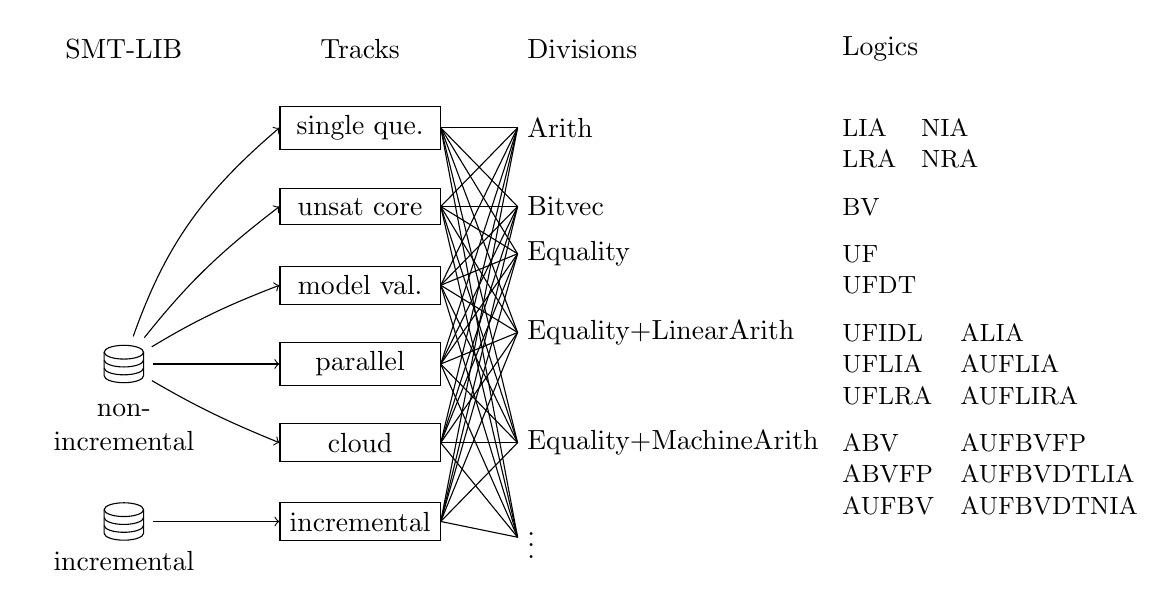
\begin{tikzpicture}
    \node at (0,6) {SMT-LIB};
    \node at (3,6) {Tracks};
    \node[anchor=west] at (5,6) {Divisions};
    \node[anchor=west] at (9,6) {Logics};

    \node[database,label=below:{\begin{tabular}{c}non-\\incremental\end{tabular}}] (nonincbench) at (0,2) {};
    \node[database,label=below:{incremental}] (incbench) at (0,0) {};

    \node[draw,text width=1.8cm,align=center](sq) at (3,5) {single que.};
    \node[draw,text width=1.8cm,align=center](uc) at (3,4) {unsat core};
    \node[draw,text width=1.8cm,align=center](mv) at (3,3) {model val.};
    \node[draw,text width=1.8cm,align=center](par) at (3,2) {parallel};
    \node[draw,text width=1.8cm,align=center](cloud) at (3,1) {cloud};
    \node[draw,text width=1.8cm,align=center](inc) at (3,0) {incremental};

    \node[anchor=west] (div1) at (5,5) {Arith};
    \node[anchor=west] at (9,5) {\small LIA};
    \node[anchor=west] at (9,4.6) {\small LRA};
    \node[anchor=west] at (10,5) {\small NIA};
    \node[anchor=west] at (10,4.6) {\small NRA};
    \node[anchor=west] (div2) at (5,4) {Bitvec};
    \node[anchor=west] at (9,4) {\small BV};
    \node[anchor=west] (div3) at (5,3.4) {Equality};
    \node[anchor=west] at (9,3.4) {\small UF};
    \node[anchor=west] at (9,3) {\small UFDT};
    \node[anchor=west] (div4) at (5,2.4) {Equality+LinearArith};
    \node[anchor=west] at (9,2.4) {\small UFIDL};
    \node[anchor=west] at (9,2) {\small UFLIA};
    \node[anchor=west] at (9,1.6) {\small UFLRA};
    \node[anchor=west] at (10.5,2.4) {\small ALIA};
    \node[anchor=west] at (10.5,2) {\small AUFLIA};
    \node[anchor=west] at (10.5,1.6) {\small AUFLIRA};
    \node[anchor=west] at (12.5,2) {$\hdots$};
    \node[anchor=west] (div5) at (5,1) {Equality+MachineArith};
    \node[anchor=west] at (9,1) {\small ABV};
    \node[anchor=west] at (9,.6) {\small ABVFP};
    \node[anchor=west] at (9,.2) {\small AUFBV};
    \node[anchor=west] at (10.5,1) {\small AUFBVFP};
    \node[anchor=west] at (10.5,.6) {\small AUFBVDTLIA};
    \node[anchor=west] at (10.5,.2) {\small AUFBVDTNIA};
    \node[anchor=west] at (12.5,1) {$\hdots$};
    \node[anchor=west] (div6)  at (5,-.2) {$\vdots$};

    \draw[->,shorten <=.3em] (nonincbench) to[bend left=15] (sq.west);
    \draw[->,shorten <=.3em] (nonincbench) to[bend left=7] (uc.west);
    \draw[->,shorten <=.3em] (nonincbench) to[bend left=5] (mv.west);
    \draw[->,shorten <=.3em] (nonincbench) to (par.west);
    \draw[->,shorten <=.3em] (nonincbench) to[bend right=4] (cloud.west);
    \draw[->,shorten <=.3em] (incbench) to (inc.west);

    \draw (sq.east) to (div1.west);
    \draw (sq.east) to (div2.west);
    \draw (sq.east) to (div3.west);
    \draw (sq.east) to (div4.west);
    \draw (sq.east) to (div5.west);
    \draw (sq.east) to (div6.west);

    \draw (uc.east) to (div1.west);
    \draw (uc.east) to (div2.west);
    \draw (uc.east) to (div3.west);
    \draw (uc.east) to (div4.west);
    \draw (uc.east) to (div5.west);
    \draw (uc.east) to (div6.west);

    \draw (mv.east) to (div1.west);
    \draw (mv.east) to (div2.west);
    \draw (mv.east) to (div3.west);
    \draw (mv.east) to (div4.west);
    \draw (mv.east) to (div5.west);
    \draw (mv.east) to (div6.west);

    \draw (cloud.east) to (div1.west);
    \draw (cloud.east) to (div2.west);
    \draw (cloud.east) to (div3.west);
    \draw (cloud.east) to (div4.west);
    \draw (cloud.east) to (div5.west);
    \draw (cloud.east) to (div6.west);

    \draw (par.east) to (div1.west);
    \draw (par.east) to (div2.west);
    \draw (par.east) to (div3.west);
    \draw (par.east) to (div4.west);
    \draw (par.east) to (div5.west);
    \draw (par.east) to (div6.west);

    \draw (inc.east) to (div1.west);
    \draw (inc.east) to (div2.west);
    \draw (inc.east) to (div3.west);
    \draw (inc.east) to (div4.west);
    \draw (inc.east) to (div5.west);
    \draw (inc.east) to (div6.west);
  \end{tikzpicture}

\end{frame}

\begin{frame}[fragile]{SMT-COMP Tracks (traditional)}
  \emph{Single Query Track}
  \begin{itemize}
  \item Determine satisfiability of one problem
  \item Solver answers sat/unsat/unknown
  \end{itemize}
  \medskip

  \emph{Unsat Core Track}
  \begin{itemize}
  \item Find small unsatisfiable subset of input.
  \item Solver answers unsat + list of formulas.
  \end{itemize}
  \medskip

  \emph{Model Validation Track}
  \begin{itemize}
  \item Find a model for a satisfiable problem.
  \item Solver answers sat + value for each non-logical symbol.
  \end{itemize}
  \medskip

  \emph{Incremental Track}
  \begin{itemize}
  \item Solve many small problems interactively.
  \item Solver acks commands and answers sat/unsat for each check.
  \end{itemize}
\end{frame}

\begin{frame}[fragile]{SMT-COMP Tracks (experimental)}

  \emph{Model Validation}
  \begin{itemize}
    \item Division with quantifier-free floating-point logics
    \item Model validation with Dolmen (thanks to Gillaume Bury and Fran\c{c}ois
    Bobot)
  \end{itemize}
  \bigskip

  \emph{Cloud and Parallel Track} (sponsored by AWS, led by Mike Whalen)
  \begin{itemize}
  \item Solve a large problem over the cloud (or a big computer)
  \begin{itemize}
    \item 100 machines, 1600 cores, 6400 GB of memory (cloud)
    \item 64 cores, 256 GB of memory (parallel)
  \end{itemize}
  \item Solver answers sat/unsat/unknown
  \end{itemize}

  \pause\bigskip

  \emph{Proof Exhibition Track}
  \begin{itemize}
  \item Solver submitted together with a checker for unsatisfiability proofs
  \item No predefined format or checker
  \item No ranking
  \item Qualitative assessment
  \end{itemize}

\end{frame}


\begin{frame}{Tracks, Solvers, Divisions, and Benchmarks}
  Teams: 21 (+3)
  \bigskip

  \begin{tabular}{c|r@{}l|r@{}l|c}
    Track & \multicolumn{2}{c|}{Solvers} & \multicolumn{2}{c|}{Divisions}  & Benchmarks \\
    \hline
    Single Query  &  22&(+3)  & 19&(+1)  & 93\,945 \\
    Incremental &  8&(+1)   & 17&(+2)  & 22\,300   \\
    Unsat Core  &  6&(-1)   & 18&(+1)  & 57\,245  \\
    Model Validation  &  8&(+1)    &  7& (+ 1 exp.)  & 32\,766  \\
    Proof Exhibition  &  &4    &  & 18 exp.  & 57\,245  \\
    \hline
    Parallel &   4&(+1)      &   &14 exp.  & 400 \\
    Cloud & 4&(-1)      &  &14 exp.  & 400 \\

  \end{tabular}
  \bigskip

  Number in parenthesis shows changes from 2021
\end{frame}

\begin{frame}
  \frametitle{Participants}

  SMT-COMP 2022 participants rely on multiple reasoning frameworks:
  \begin{itemize}
  \item CDCL(T)
  \item mcSAT
  \item saturation
  \item automata
  \item finite domain
  \item CP
  \item local search
  \item besides wrappers extending the scope of existing solvers
  \end{itemize}

  \bigskip
  Six new solvers participated:
  \begin{itemize}
  \item NRA-LS   {\footnotesize (Liu et al.)}
  \item OSTRICH {\footnotesize (Chen et al.)}
  \item Q3B {\footnotesize (Jon\'a\v{s} and Strej\v{c}ek)}
  \item Yices-ismt {\footnotesize (Jia et al.)}
  \item Z3++ {\footnotesize (Cai et al.)}
  \item solsmt {\footnotesize (Reitwiessner and Soos)}
  \end{itemize}

\end{frame}


\begin{frame}
  \frametitle{Non-Competitive Solvers}

  Submitted by organisers
  \begin{itemize}
  \item z3-4.8.17
  \item MathSAT 5.6.8
  \item Division winners from previous years (23 Solvers)
  \end{itemize}
  \bigskip

  Submitted by participants
  \begin{itemize}
  \item Fixed solvers (OpenSMT, STP, Yices-ismt, Z3++,smtinterpol)
  \end{itemize}
\end{frame}


\begin{frame}{Scoring}
  Computing scores:
  \begin{itemize}
  \item \emph{Single Query/Parallel/Cloud}: number of solved \emph{instances}
  \item \emph{Incremental}: number of solved \emph{queries}
  \item \emph{Unsat Core}: number of top-level assertions \emph{removed}
  \item \emph{Model Validation}: number of solved instances with correct \emph{models}
  \end{itemize}

  \bigskip
  Error scores:
  \begin{itemize}
  \item \emph{All Tracks}: given for sat reply for unsat instance, or vice versa
  \item \emph{Unsat Core}: given if returned core is satisfiable.
  \item \emph{Model Validation}: given if given model evaluates formula to \emph{false}
  \end{itemize}
  Error scores are draconian.
\end{frame}

\begin{frame}{Score and Ranking}
  In each track we collect different scores:
  \begin{itemize}
  \item \emph{Sequential score} (SQ, UC, MV): all time limits apply to cpu time
  \item \emph{Parallel score} (all): all time limits apply to wallclock time
  \item \emph{SAT score} (SQ): parallel score for \emph{satisfiable} instances
  \item \emph{UNSAT score} (SQ): parallel score for \emph{unsatisfiable} instances
  \item \emph{24s} (SQ): parallel score with time limit of \emph{24s}
  \end{itemize}
  \bigskip

  Division ranking (for each score)
  \begin{itemize}
  \item For each division, one winner is declared
  \end{itemize}

  \bigskip

  Two competition-wide rankings (for each score)
  \begin{itemize}
  \item \emph{Biggest lead}: division winner with most score difference to second place
  \item \emph{Largest contribution}: improvement each solver provided to a virtual best solver
  \end{itemize}

\end{frame}

\begin{frame}{FLoC Medalists}

  \begin{columns}
    \begin{column}{0.6\textwidth}

  \Large 8 medals
  \begin{itemize}
    \bigskip
    \vitem Biggest Lead
    \begin{itemize}
      \item Single Query: Gold and Silver
      \item Model Validation: Gold
      \item Incremental: Gold
    \end{itemize}
    \bigskip

    \vitem Largest Contribution
    \begin{itemize}
      \item Single Query: Gold and Silver
      \item Model Validation: Gold
      \item Incremental: Gold
    \end{itemize}
  \end{itemize}
\end{column}
\hfill
\begin{column}{0.4\textwidth}
  \begin{center}
    \includegraphics[width=.3\textwidth]{medalgold}
    \includegraphics[width=.3\textwidth]{medalgold}
    \includegraphics[width=.3\textwidth]{medalgold}
    \includegraphics[width=.3\textwidth]{medalgold}
    \includegraphics[width=.3\textwidth]{medalgold}
    \includegraphics[width=.3\textwidth]{medalgold}\\
    \includegraphics[width=.3\textwidth]{medalsilver}
    \includegraphics[width=.3\textwidth]{medalsilver}
  \end{center}
\end{column}
\end{columns}

\end{frame}

\begin{frame}{FLoC Medalists}

  \begin{columns}
    \begin{column}{0.6\textwidth}

  \Large cvc5 wins three gold medals:
  \begin{itemize}
    \bigskip
    \vitem Single Query, Biggest Lead
    \bigskip

    \vitem Single Query, Largest Contribution
    \bigskip

    \vitem Incremental, Largest Contribution
  \end{itemize}
\end{column}
\hfill
\begin{column}{0.4\textwidth}
  \begin{center}
    \includegraphics[width=.3\textwidth]{medalgold}
    \includegraphics[width=.3\textwidth]{medalgold}
    \includegraphics[width=.3\textwidth]{medalgold}
  \end{center}
\end{column}
\end{columns}

\end{frame}

\begin{frame}{FLoC Medalists}

  \begin{columns}
    \begin{column}{0.6\textwidth}

  \Large Z3++ wins two gold medals:
  \begin{itemize}
    \bigskip
    \vitem Model Validation, Biggest Lead
    \bigskip

    \vitem Model Validation, Largest Contribution
  \end{itemize}
\end{column}
\hfill
\begin{column}{0.4\textwidth}
  \begin{center}
    \includegraphics[width=.3\textwidth]{medalgold}
    \includegraphics[width=.3\textwidth]{medalgold}
  \end{center}
\end{column}
\end{columns}

\end{frame}

\begin{frame}{FLoC Medalists}

  \begin{columns}
    \begin{column}{0.6\textwidth}

  \Large SMTInterpol wins one gold medal:
  \begin{itemize}
    \bigskip
    \vitem Incremental, Biggest Lead
  \end{itemize}
\end{column}
\hfill
\begin{column}{0.4\textwidth}
  \begin{center}
    \includegraphics[width=.3\textwidth]{medalgold}
  \end{center}
\end{column}
\end{columns}

\end{frame}

\begin{frame}{FLoC Medalists}

  \begin{columns}
    \begin{column}{0.6\textwidth}

  \Large Bitwuzla wins one silver medal:
  \begin{itemize}
    \bigskip
    \vitem Single Query, Biggest Lead
  \end{itemize}
\end{column}
\hfill
\begin{column}{0.4\textwidth}
  \begin{center}
    \includegraphics[width=.3\textwidth]{medalsilver}
  \end{center}
\end{column}
\end{columns}

\end{frame}

\begin{frame}{FLoC Medalists}

  \begin{columns}
    \begin{column}{0.6\textwidth}

  \Large YicesQS wins one silver medal:
  \begin{itemize}
    \bigskip
    \vitem Single Query, Largest Contribution
  \end{itemize}
\end{column}
\hfill
\begin{column}{0.4\textwidth}
  \begin{center}
    \includegraphics[width=.3\textwidth]{medalsilver}
  \end{center}
\end{column}
\end{columns}

\end{frame}

\begin{frame}

  \begin{center}
    \Large For full results please come to the SMT workshop Thursday 4pm.
  \end{center}

\end{frame}

\end{document}
